\documentclass{refrep}
\settextfraction{.9}
\usepackage{extramarks}
\usepackage{amsmath}
\usepackage{amsthm}
\usepackage{amsfonts}
\usepackage{tikz}
\usepackage[plain]{algorithm}
\usepackage{algpseudocode}
\usepackage{listings}
\usepackage{datetime}
\usepackage{xcolor}
\usepackage{float}
\usepackage{graphicx}
\usepackage[export]{adjustbox}
\usepackage{caption}
\usepackage{contour}
\usepackage{longtable}
\makeatletter
\newcount\dirtree@lvl
\newcount\dirtree@plvl
\newcount\dirtree@clvl
\def\dirtree@growth{
  \ifnum\tikznumberofcurrentchild=1\relax
  \global\advance\dirtree@plvl by 1
  \expandafter\xdef\csname dirtree@p@\the\dirtree@plvl\endcsname{\the\dirtree@lvl}
  \fi
  \global\advance\dirtree@lvl by 1\relax
  \dirtree@clvl=\dirtree@lvl
  \advance\dirtree@clvl by -\csname dirtree@p@\the\dirtree@plvl\endcsname
  \pgf@xa=.25cm\relax
  \pgf@ya=-.5cm\relax
  \pgf@ya=\dirtree@clvl\pgf@ya
  \pgftransformshift{\pgfqpoint{\the\pgf@xa}{\the\pgf@ya}}%
  \ifnum\tikznumberofcurrentchild=\tikznumberofchildren
  \global\advance\dirtree@plvl by -1
  \fi
}

\tikzset{
  dirtree/.style={
    growth function=\dirtree@growth,
    every node/.style={anchor=north},
    every child node/.style={anchor=west},
    edge from parent path={(\tikzparentnode\tikzparentanchor) |- (\tikzchildnode\tikzchildanchor)}
  }
}

\makeatother
\graphicspath{ {images/vc707/} {images/vc709/} {images/qsys/} {images/ipc/} {images/perf/} {images/}}
\newcommand{\TinkerVersion}{Tinker 1.0 (Beta)}
\newcommand{\figurewidth}{350px}
\newcommand{\Directory}[1]{\textit{#1}}
\newcommand{\EnvVariable}[1]{\textbf{#1}}
\newcommand{\TermCmd}[1]{\$ \texttt{#1}}
\newcommand{\TODO}[1]{\textbf{\color{red}{#1}}}
\newcommand{\Altera}[1]{{\color{blue}{#1}}}
\newcommand{\ConfigSetting}[1]{\textbf{#1}}

\title{{\TinkerVersion} Documentation}
\author{Dustin Richmond}
\date{\today}

\begin{document}

\maketitle
\pagebreak
\tableofcontents

\chapter{Introduction: Tinker}
\label{Chapter:Intro}
\section{Licensing}

Copyright (c) 2016, The Regents of the University of California All rights
reserved.

Redistribution and use in source and binary forms, with or without modification,
are permitted provided that the following conditions are met:

\begin{itemize}
    \item Redistributions of source code must retain the above copyright
      notice, this list of conditions and the following disclaimer.

    \item Redistributions in binary form must reproduce the above
      copyright notice, this list of conditions and the following
      disclaimer in the documentation and/or other materials provided
      with the distribution.

    \item Neither the name of The Regents of the University of California
      nor the names of its contributors may be used to endorse or
      promote products derived from this software without specific
      prior written permission.
\end{itemize}

THIS SOFTWARE IS PROVIDED BY THE COPYRIGHT HOLDERS AND CONTRIBUTORS ``AS IS''
AND ANY EXPRESS OR IMPLIED WARRANTIES, INCLUDING, BUT NOT LIMITED TO, THE
IMPLIED WARRANTIES OF MERCHANTABILITY AND FITNESS FOR A PARTICULAR PURPOSE ARE
DISCLAIMED. IN NO EVENT SHALL REGENTS OF THE UNIVERSITY OF CALIFORNIA BE LIABLE
FOR ANY DIRECT, INDIRECT, INCIDENTAL, SPECIAL, EXEMPLARY, OR CONSEQUENTIAL
DAMAGES (INCLUDING, BUT NOT LIMITED TO, PROCUREMENT OF SUBSTITUTE GOODS OR
SERVICES; LOSS OF USE, DATA, OR PROFITS; OR BUSINESS INTERRUPTION) HOWEVER
CAUSED AND ON ANY THEORY OF LIABILITY, WHETHER IN CONTRACT, STRICT LIABILITY, OR
TORT (INCLUDING NEGLIGENCE OR OTHERWISE) ARISING IN ANY WAY OUT OF THE USE OF
THIS SOFTWARE, EVEN IF ADVISED OF THE POSSIBILITY OF SUCH DAMAGE.
\section{What is Tinker}
\section{Understanding this User Guide}
In this user guide, we use the following conventions:
\begin{center}
  \begin{tabular}{ | l | l |}
    \hline
    Object & Example \\ \hline
    Directories and Paths & \Directory{tinker/boards/14.1}  \\ \hline
    Configuration Setting & \ConfigSetting{Number of Lanes} \\ \hline
    Terminal Command, Code Snippet & \TermCmd{echo ``Hello World''}\\ \hline
  \end{tabular}
\end{center}

\section{Decoding What's Provided}
\label{Chapter:Intro:Sec:Decoding}
Fig~\ref{Fig:Tinker:DirStructure} shows the directory hierarchy of RIFFA. This
instruction manual uses this directory tree when specifying all directory paths.

\begin{itemize}
\item \Directory{boards/} contains all of boards supported by tinker, grouped by Quartus Version
\item \Directory{docs/} contains all of the documentation for this project
\item \Directory{example/} contains a set of example user specifications (written in JSON)
\item \Directory{python/} contains all of the Python files necessary for running tinker
\item \Directory{tcl/} contains all of the tcl scripts used by Quartus/Qsys during OpenCL Compilation
\item \Directory{tests/} contains a set of tests that can be used to test a custom board. 
\end{itemize}

\begin{figure}[H]
  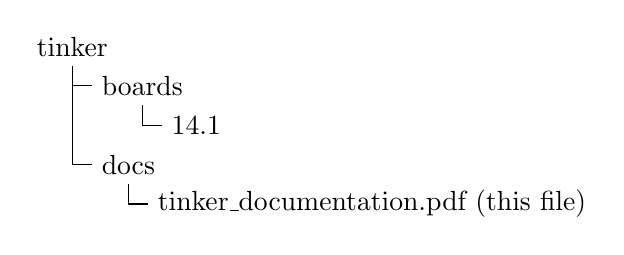
\begin{tikzpicture}[dirtree]
    \node {tinker}
    child { 
      node {boards}
      child { 
        node {14.1} 
      }
    }
    child { 
      node {docs}
      child { 
        node {tinker\_documentation.pdf (this file)}
      }
    };
  \end{tikzpicture}
  \caption{Directory hierarchy of the RIFFA \TinkerVersion~distribution} \label{Fig:Tinker:DirStructure}
\end{figure}

\section{Release Notes}
\subsection{Tinker 1.0 (Beta)}
\begin{itemize}
  \item Beta Release: There may be bugs in this version. 
  \item Support for Terasic DE5Net Board in Quartus 14.1
\end{itemize}
\pagebreak
\chapter{Setup and Installation}
\label{Chapter:Setup}
\section{Dependencies}
% TODO: TCLXML, Python, Quartus, Linux
\section{Environment}
% TODO: Set Environment Variables: TCLXML_PATH TINKER_PATH
\pagebreak
\chapter{Generating and Compiling a Custom Board}
\label{Chapter:Generating}
\section{Running the Board Generation Utility tinker}
\label{Chapter:Generating:Sec:Tinker}
\section{Custom Board Installation}
\label{Chapter:Generating:Sec:Installation}
\section{Custom Board Compilation}
\label{Chapter:Generating:Sec:Compilation}
\pagebreak
\chapter{Adding Support a New Board}
\label{Chapter:Adding}
\section{Top Level Design File}
\label{Chapter:Adding:Section:Top}
\section{Board XML File}
\label{Chapter:Adding:Section:XML}

\section{Project File}
\label{Chapter:Adding:Section:Project}
\section{Timing Files}
\label{Chapter:Adding:Section:Timing}
\subsection{Memory Interfaces}
\label{Chapter:Adding:Section:Project:Sub:Memories}
\section{Qsys Files}
\label{Chapter:Adding:Section:Qsys}
% Kernel Interface
\section{Installation}
\label{Chapter:Adding:Section:Installation}
\section{Testing}
\label{Chapter:Adding:Section:Testing}
\pagebreak
\chapter{Developer Documentation}
\label{Chap:Tinker:Adding}
\end{document}
